\documentclass{article}
\newcommand{\tab}[1]{\hspace{.2\textwidth}\rlap{#1}}

\usepackage[margin=1in]{geometry}
\usepackage[parfill]{parskip}
\usepackage{graphicx}

\setlength{\parindent}{.5in}

\begin{document}



\centerline{\sc \large Code Camp Challenge v5.0}
\vspace{.5pc}
\centerline{\sc Bell Tower Escape!}
\vspace{2pc}

\section*{Background}
Soon after Jurassic Park re-opened, some of the dinosaurs were purchased by the Pillsbury family for a Minneapolis branch of Jurassic Park. Unfortunately, they escaped and have made their way to the GMI campus. During an East Wing wide meeting on every floor of the Bell Tower involving network latency, the dinosaurs started getting in...! Due to the inciting panic, and velociraptors taking over the lower levels of the stair well (the doors only open inwards - so there's nothing to worry about!), the Bell Tower Elevators have been overloaded with people trying to get away from the trapped velociraptors and other people trying to get out of the building - as such, they need to be reprogrammed.

Each bank of the elevators are controlled by a different micro-controller, and elevator engineers have asked you to program one of them, and another colleague to program the other. They figured one of your algorithms will be efficient enough to get everyone where they want on time!

\section*{Game Information}
You get to control two elevators that go up and down the twelve floors. You know what floor people are on and find out what floor they are trying to get to once they enter your elevator. Each turn consists of either moving an elevator up a floor, down a floor, or allowing people to get on or off (people will get on and off in the same turn). If an elevator from both banks opens on the same floor, the group will go for the elevator with fewer people, until the elevator's capacity is met, then people will go into a different elevator.

The game is turn based with 500 turns and the person who has `delivered' the most amount of people in that time is declared the winner. When people get on your elevator, they will have a `patience' value that starts at $$abs(destFloor-currentFloor) * frustrationCoefficient + 3$$ where $frustrationCoefficient = 2$. This value decreases by 1 every turn and if it's negative the Meeple will get off at the next elevator stop and count negatively towards the number of people delivered.

\section*{Submission}
To submit your AI, place a folder with your name on it in \verb|\\genmills.com\corportate\PUBLIC\codecamp| by midnight on Monday July 20th. We ask that you submit a working Windows binary with the endpoint set to http://localhost:3193/, along with your source code and any special build/run instructions (especially if you created a custom agent).

\section*{Issues}
For any issues, please create an issue on our GitHub page (https://github.com/eonarheim/BellTowerEscape). If you have any questions feel free to reach out to Erik Onarheim or Shakil Thakur, and they will rather enthusiastically discuss anything.

\section*{Setting it up}
\begin{enumerate}
\item If you're familiar with git: \verb|git clone http://github.com/eonarheim/BellTowerEscape| otherwise head over to http://github.com/eonarheim/BellTowerEscape and click on `Download Zip' from the right side of the menu.

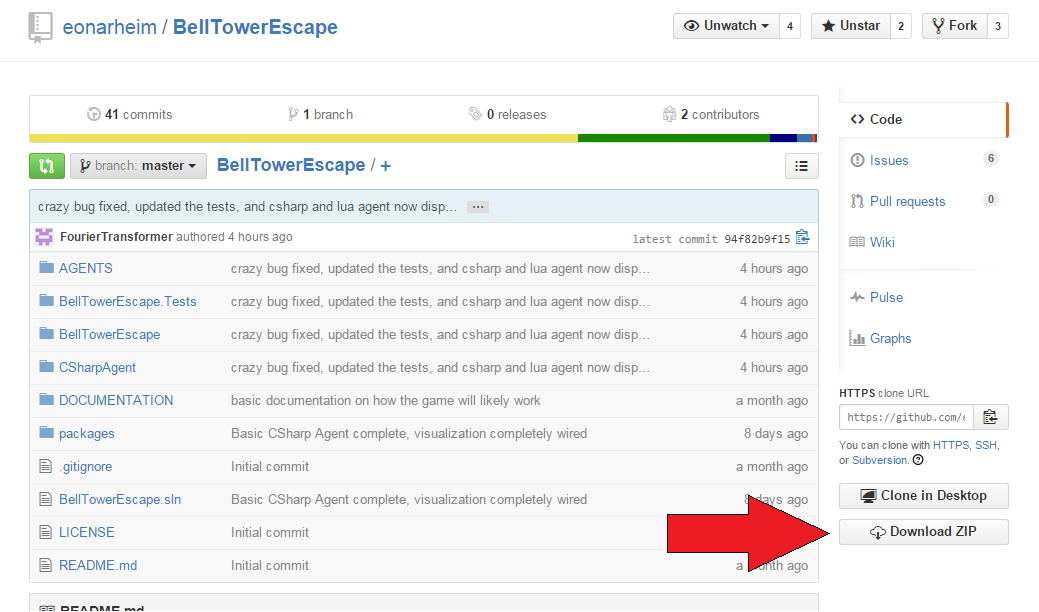
\includegraphics[width=6.5in]{1-DownloadZip.png}

\item Open up \verb|BellTowerEscape.sln| in Visual Studio. If you don't have an MSDN license, you should be able to use the Community Edition of Visual Studio (https://www.visualstudio.com/en-us/products/visual-studio-community-vs.aspx) to run the code. It might also run in Visual Studio Code, but we haven't explored that territory yet. If you try it and get it working let us know!

\item Visual Studio will likely want to get some packages or update some things. Just kind of let it do its thing. If you need some help, reach out to someone in App Dev and they'll likely be more than happy to help out!

\item Click on `BellTowerEscape' in the Solution Explorer and the little Play button to build it and use the little drop-down to launch it in your favorite browser. It might start doing a `Nuget Package Restore'. Again, just let Visual Studio do its thing.

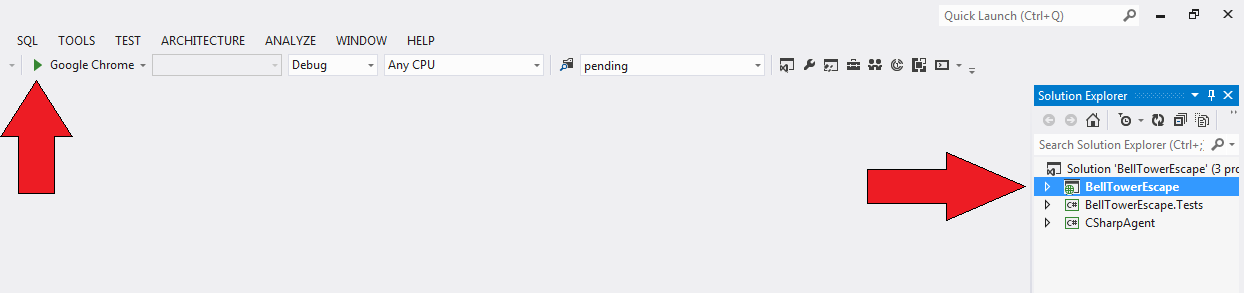
\includegraphics[width=6.5in]{4-BuildIt.png}
\newpage
\item Once it's loaded up and you can see the web page built, you can start up an agent! The easiest one to get going is the CSharp agent. All you have to do is Right-click `CSharpAgent' in the solution explorer, click on `Debug' and then `Start new instance' and that should get it going!

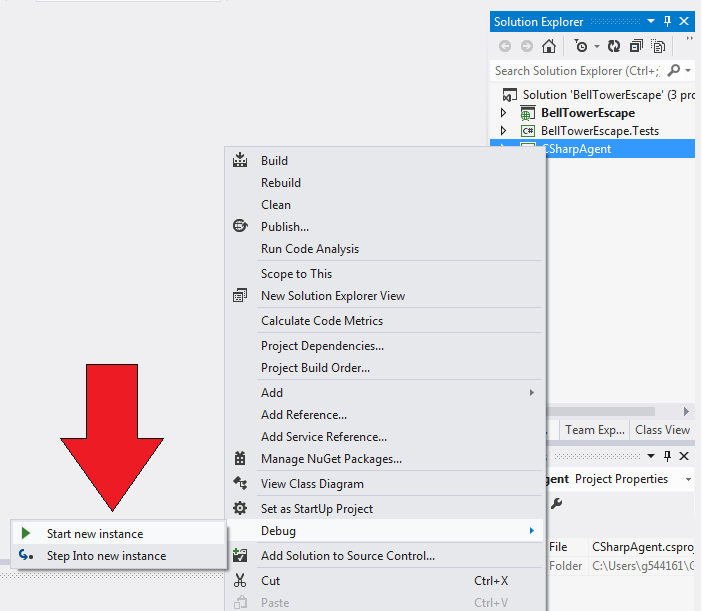
\includegraphics[width=4.5in]{5-CSharp.png}

\item SWEET! Now that you got it running, I'm sure you want to make some changes! Click the little drop-down next to `CSharpAgent' and open up `Agent.cs'. This file should be all you need to modify to create your own AI.

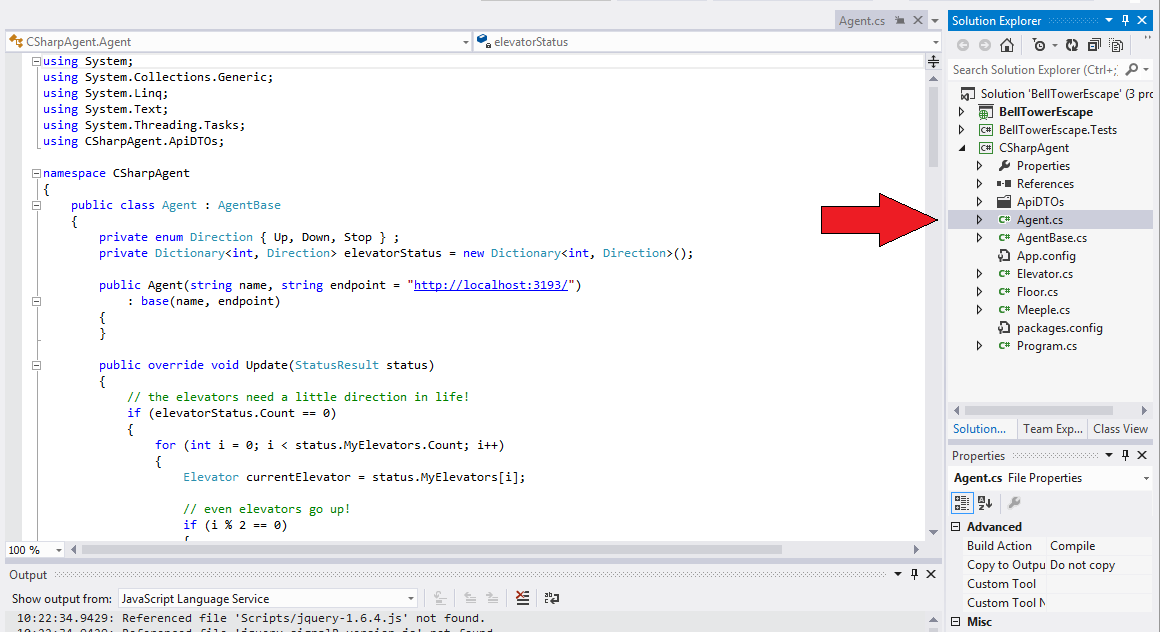
\includegraphics[width=6.5in]{6-AgentCS.png}

The code that's currently there is the default agent code that's equivalent to the one on the server. It's doing the Elevator Sweep Algorithm similar to what most elevators use today. This algorithm could be improved upon or scrapped entirely for something new, but exists to show how to interact with game server and is the default agent that you will play against when testing your code.

\end{enumerate}

\subsection*{The Elevator Sweep Algorithm}
Each elevator is set to move up or down. As it goes in that direction, if there are other people to pick up who also want to go in that direction, those people are picked up! It then continues dropping people off until it reaches the highest/lowest floor, switches direction, and then continues. This is similar to how non-smart elevators work today.

We've also provided a Lua and Python agent which can be found in the `Agents' folder of the solution and we have some READMEs there to help get you going on those!

\section*{THE COMPETITION}
Once we've gathered all the submissions we'll pit them against one another and determine who has the best AI of them all!

\end{document}